% !TEX encoding = UTF-8 Unicode
%!TEX root = ../Main/thesis.tex
% !TEX spellcheck = en-US
%%=========================================
\documentclass[../Main/thesis.tex]{subfiles}
\begin{document}
\chapter[Application of the High frequency resonance technique in bearing Fault detection]{Application of the High frequency resonance technique in bearing Fault detection}
\label{sec:chapter2}
This chapter covers the application of the high frequency resonance technique (HFRT), to bearing fault detection. It starts with the background materials in section \ref{sec:background-material}, where section \ref{sec:fouurier-analysis} presents an overview of the Fourier analysis, while section \ref{sec:filters} describes signal filtering operations such as the Hilbert transform, low and band pass filtering. 
\justify
It should be noted that the Hilbert transform filters out negative frequencies, per its application in the high frequency resonance technique. Beyond that, it is an important tool in the Hilbert Huang transform, in analyzing signals with modulated spectral characteristics. Regarding the low pass filter, it removes high frequencies components of a signal, while a band pass filter get ride of signal components below and above predefined threshold values.
\justify
After discussing the background materials, section \ref{sec:application} describes a case study where the high frequency resonance technique is applied to detecting bearing failure frequencies. The data for this case study, was provided by the intelligence system division, of the national aeronautics and Space administration (NASA), and is the subject of divers scientific publications.

\section{Background materials}
\label{sec:background-material}
\subsection{Fourier analysis}
\label{sec:fouurier-analysis}
From solving differential equations to analyzing sound waves, images and signals in general, Fourier analysis has a profound impact in science and engineering. It provides a convenient way to transforming signals into a series of frequencies called frequency spectrum. And in doing so, it reveals hidden aspects of data. The bulk of Fourier analysis is to decompose as well as reconstruct a signal, or more generally a function, into trigonometric extensions. In bearing fault detection, the main goal is to decompose a signal into its elementary frequency spectrum, which contains the bearing defect frequencies, if they exist. 
\justify
  In an application view point, a signal can be viewed as a series of observations generated by a given process, and recorded at discrete or continuous time intervals. The underlying process might be the sum of given sub-processes. In this case, the frequency spectrum will reveal all the sub-processes characteristics.
This is illustrated in Figure \ref{fig:fft_domain}, where a signal (in dark) is decomposed into four sinusoidal components (in blue). Each sinusoidal component is uniquely defined by its amplitude and its frequency (in red). The representation of all amplitudes versus their corresponding frequencies is called the frequency spectrum.
%The sinusoidal components can be represented in a coordinate system with frequencies on the x axe and amplitudes on the y axe (in red). This is called the frequency domain. From the frequency domain we can observe a hight amplitude low frequency component. As we move toward high frequencies, the amplitudes decrease.
\begin{figure}[H] %  figure placement: here, top, bottom, or page
   \centering
   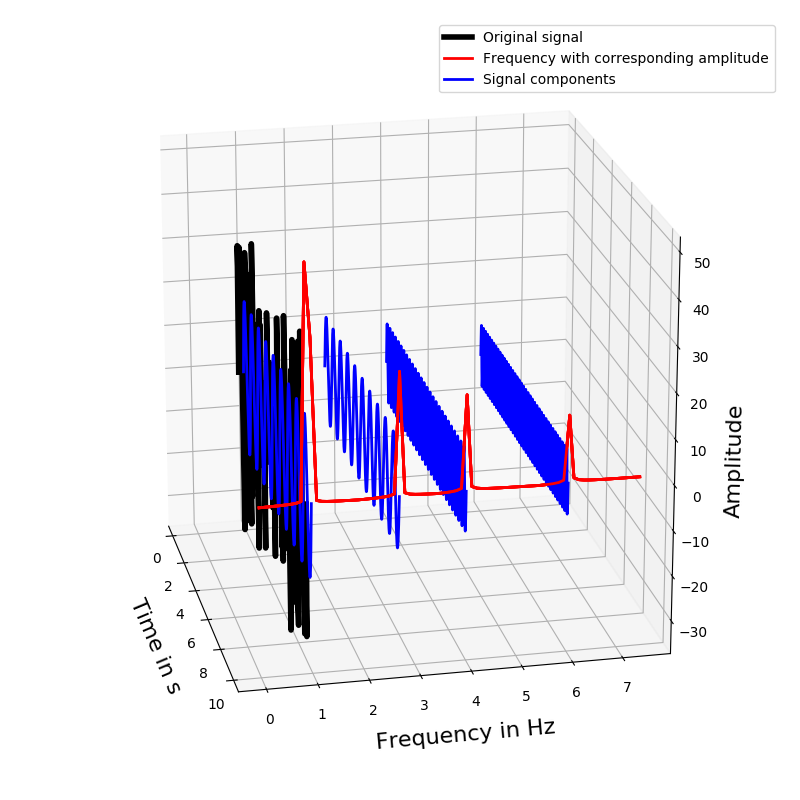
\includegraphics[width=6in]{../fig/fft_domain} 
   %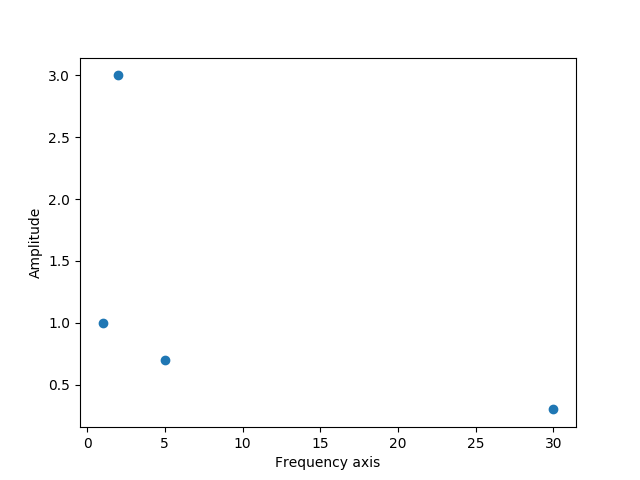
\includegraphics[width=2.5in]{freq} 
   \caption{}
   \label{fig:fft_domain}
\end{figure}
\justify
In a theoretical view point, however, the results that underlie Fourier analysis can be sum up as followed: Given a function (or a signal), find a trigonometric series that converges to the target function. The latter statement falls under the umbrella of the general problem of function approximation.  
\justify
The basic ingredients required to approximate a function in this scenario are: a vector space, a basis, which is a subspace of the vector space, and a mathematical operation such as an inner product that maps two vectors to a real number. If a vector space has an inner product, we say that the vector space is an inner product space. The inner product operation, can be used for example to express the orthogonality property. The latter plays an import part in simplifying some algebraic operations.
\justify
Before continuing, let clarify some symbols. In this section, the letters $f$, $V$, $V_{0}$ are used for an arbitrary function, a vector space, and a subspace of a vector space, respectively.
Basis functions will be denoted by $\{  \varphi_{0}, \cdots,\varphi_{n}\}$, where $n$ can either be a finite integer or infinite. Having made this clarification, let elaborate on the concept of function approximation. 
\justify
The function approximation process in light of Fourier analysis goes like this: Given an arbitrary function $f$, that is to be approximated, pick an appropriate vector space $V$, such that $f\in V$. Furthermore, define a subspace $V_{0}$ of the vector space $V$, and construct an inner product on $V_{0}$, if it does not exist. Next, fine an appropriate basis of $V_{0}$.  A basis of $V_{0}$ is a set of linearly independent vectors   $\{  \varphi_{0}, \cdots,\varphi_{n}\}$ in $V_{0}$, that span $V_{0}$. This means that any vector in $V_{0}$ can be written as a linear combination of the basis vectors.
\justify
 Having all this in place, the best approximation of the function $f$ is its orthogonal projection in the inner product space $V_{0}$. Figure \ref{figure:il} shows an illustration of a generic mechanism of function approximation by orthogonal projection, where $f_{0}$ is the orthogonal projection of $f$ in the subspace $V_{0}$ of $V$.
\justify
\begin{figure}[H]
\begin{center}
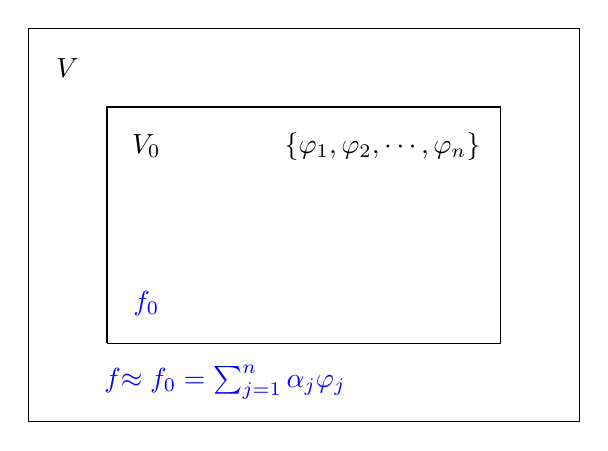
\begin{tikzpicture}
\path (0,0) coordinate (origin1);
\path(0.5,4.5) node (V){$V$};
\path(2.5,0.5) node (f){$\textcolor{blue}{f}\textcolor{blue} {\approx f_{0} = \sum_{j=1}^{n} \alpha_{j} \varphi_{j}}$};
\path (0,5) coordinate (topleft1);
\path (7,5) coordinate (topright1);
\path (7,0) coordinate (bottom1);
% draw
\draw (origin1) -- (bottom1) -- (topright1) -- (topleft1) -- (origin1);

% reactagle 2
\path (1,1) coordinate (origin2);
\path(1.5,3.5) node (V0){$V_{0}$};
\path(1.5,1.5) node (f0){$\textcolor{blue}{f_{0}}$};

\path (1,4) coordinate (topleft2);
\path (6,4) coordinate (topright2);
\path(4.5,3.5) node (b0){$ \{\varphi_{1}, \varphi_{2}, \cdots, \varphi_{n}\} $};
\path (6,1) coordinate (bottom2);
% draw
\draw (origin2) -- (bottom2) -- (topright2) -- (topleft2) -- (origin2);
\end{tikzpicture}
\end{center}
\caption{Illustration of a generic function approximation process of a function $f$ into a subspace $V_{0}$ of a vector space $V$. $\varphi_{j}$ are the basis functions and $\alpha_{j}$ are real numbers for $j=1,\cdots,n$.}
\label{figure:il}
\end{figure}

\justify
Having the generic function approximation defined in Figure \ref{figure:il} as a blue print, the Fourier space $V_{0}$ is a subspace of the space of all continuous functions of the interval $[0, T]$ and denoted by $C[0,T] $, which is $V$ in Figure \ref{figure:il}. The subspace $V_{0}$ of $V$ is spanned by 
\begin{equation}
\left\{1, \cos\left( \frac{2\pi t}{T} \right), \cdots,\cos\left( \frac{2\pi Nt}{T} \right), \sin\left( \frac{2\pi t}{T} \right), \cdots,\sin\left( \frac{2\pi Nt}{T} \right)   \right\}. \nonumber
\end{equation}
which corresponds to
\begin{equation}
\{\varphi_{1}, \varphi_{2}, \cdots, \varphi_{n}\}, \nonumber
\end{equation}
from figure \ref{figure:il}. 
\justify
Let sum up this introductory section of Fourier analysis. Fourier analysis is concerned with the general problem of periodic and non periodic functions approximation. The former and the latter are treated by Fourier series and Fourier transform, respectively. Given a periodic function, its Fourier series is given as a discrete superposition of trigonometric functions, and its Fourier transform is expressed as continuous superposition of exponential functions.
To extend the discussion of Fourier analysis, section \ref{sec:fouurier-serie} presents the Fourier series, while section \ref{sec:fouurier-transform} elaborates on Fourier transform. In section \ref{sec:application}, the application of Fourier analysis to bearing fault detection is presented.

\justify
\subsubsection{Fourier series}
\label{sec:fouurier-serie}
 Let $f$ be an arbitrary function, defined on an interval of length $L = \pi$. Its Fourier series representation is given by the infinite series
\begin{equation}\label{eq:fs}
f(t) = \frac{a_{0}}{2} +\sum_{n=1}^{\infty}\left( a_{n} \cos\left( \frac{n\pi t}{L}\right) + b_{n} \sin\left( \frac{n\pi t}{L}\right)  \right),
 \end{equation}
where the coefficients $a_{0}, a_{1}, \cdots, b_{1}, b_{2},\cdots$, corresponding to the $\alpha_{j}$ in Figure \ref{figure:il}, are given by 
\begin{equation}\label{eq:fsc}
\begin{split}
a_{n} &= \frac{1}{L}\int_{-L}^{L}f(t)\cos\left( \frac{m\pi t}{L}\right) \mathrm{d}t,\quad n=0,1,2,\cdots\\
b_{n} &= \frac{1}{L}\int_{-L}^{L}f(t)\sin\left( \frac{n\pi t}{L}\right) \mathrm{d}t,\quad n=1,2,\cdots
\end{split}
\end{equation}
 Approximating a function by an infinite series such as in equation (\ref{eq:fs}), raises few interesting questions. The right hand side of (\ref{eq:fs}) being an infinite series, must obviously converge for this expression to be valid. As such, under which condition does it converge? and what type of convergence is required? what are the characteristics of the function that it converges to?.
\justify
At first glance, one can observe that the trigonometric functions in the infinite series are periodic with period $2L$. This suggests that the class of functions admitting a Fourier series must be periodic, with period $2L$. The second observation is that the trigonometric extensions are continuous, therefore some sort of continuity property must be imparted on the function $f$. It turns out that, the convergence of Fourier series and the characteristics of the function $f$ are intimately tied. This is formerly expressed in the following theorem
\begin{theorem}\label{thm:conv}
	The function $f(t)$ will  have a convergent Fourier series, with coefficients given by (\ref{eq:fsc}), provided $f(t)$ is periodic with period $2L$, and both $f(t)$ and $f^{\prime}(t)$ (the derivative of $f(t)$) are at least piecewise continuous.
\end{theorem}
\justify
A useful interpretation of what it means for a function $f(t)$ to have a Fourier representation, can be expressed in terms of the partial sum
\begin{equation}\label{eq:ps}
	S_{N} = \frac{a_{0}}{2} +\sum_{n=1}^{N}\left( a_{n} \cos\left( \frac{n\pi t}{L}\right) + b_{n} \sin\left( \frac{n\pi t}{L}\right)  \right).
\end{equation}\label{eq:ps1}
The function $f(t)$ has a Fourier representation given by (\ref{eq:fs}) means that 
\begin{equation}\label{eq:ps1}
\lim_{N\rightarrow\infty}S_{N}(t)= f(t)
\end{equation}
where N is an integer. 
\justify
Theorem \ref{thm:conv} ensures that if a function is periodic, and both the function and it first derivative are piecewise continuous, then it will have a convergence Fourier transform. Now, the question which remains to be addressed is, what type of convergence should be expected? The convergence type of Fourier series discussed in this section are: uniform convergence, pointwise convergence and mean-square convergence. The two first convergence type deal with continuous functions, while mean-square convergence treats discontinuous functions. 
\justify
Uniform convergence is more stringent than pointwise convergence, while pointwise convergence is more strict than mean-square convergence. Specifically, uniform convergence implies pointwise convergence, and pointwise convergence implies mean-square convergence. Therefore, together, they form a hierarchy of convergence type. 
\justify
In terms of function approximation, convergence of infinite series starts with examining the error incurred by approximating the function by the infinite series. This error is expressed as 
\begin{equation}\label{eq:error}
E_{N}(t) = f(t)-S_{N}(t) = \sum_{n=N+1}^{\infty}\left( a_{n} \cos\left( \frac{n\pi t}{L}\right) + b_{n} \sin\left( \frac{n\pi t}{L}\right)  \right).
\end{equation} 
It is now apparent that the Fourier series converges pointwise to $f(t)$ if and only if 
\begin{equation}
\lim_{N\rightarrow\infty}E_{N}(t)= 0\quad \text{for all $t$}.
\end{equation}
Pointwise convergence can also be formulated in terms of the series in equations (\ref{eq:ps}, \ref{eq:ps1}). Formally, the sequence $S_{N}$ converges pointwise if for some fixed $t$ and fixed $\epsilon$ (a small real number), it exists some $M\in \mathbb{Z}$, such that for $N\geq M$
\begin{equation}
\abs{S_{N}(t)-f(t)} \leq \epsilon.
\end{equation}
All the previous discussions can be summarized in the following theorem
\begin{theorem}
	if $f$ is differentiable on $[-\pi, \pi]$ then the Fourier series converges pointwise
	and \ref{eq:fs} holds at every point $t$ where $f(t)$ is continuous.
\end{theorem}
Now let turn our attention to uniform convergence.
since the trigonometric functions in the infinite Fourier series are bounded above by 1, we can write 
\begin{equation}
\abs{E_{N}(t)} \leq \sum_{n = N+1}^{\infty} \left(\abs{a_{n}} + \abs{b_{n}}\right),
\end{equation} 
and provided that the left hand side converges, uniform convergence is warranted. This is summed up in the following theorem
\begin{theorem}
	The Fourier series for $f(t)$ converges uniformly, and therefore $f(t)$ is continuous if
	 \begin{equation}
	  \sum_{n = N+1}^{\infty} \left(\abs{a_{n}} + \abs{b_{n}}\right),
	 \end{equation}
	 converges
\end{theorem}
Since a discontinuous function can not have a uniform convergence Fourier series, what should be expected from discontinuous function in terms of convergence? this question can be answered in terms of mean-square convergence.
The mean-square value of the approximation error $E_{N}(t)$, also interpreted physically as the average energy of the approximation error $E_{N}(t)$ (define in equation (\ref{eq:error})) in the interval of length $L$, is given by 
\begin{equation}\label{eq:mc}
	\frac{1}{2L}\int_{-L}^{L}\left(E_{N}(t)\right)^{2}\mathrm{dt} = \frac{1}{2}\sum_{n=N+1}^{\infty}\left(a_{n}^{2} + b_{n}^{2}\right).
\end{equation}
If the right hand side of equation (\ref{eq:mc}) converges then 
\begin{equation}
	\lim_{N\rightarrow \infty}\left( \frac{1}{2L}\int_{-L}^{L}\left(E_{N}(t)\right)^{2}\mathrm{dt}  \right) = 0.
\end{equation}
This result can be formulated in the following theorem.
\begin{theorem}\label{thm:msc}
	The Fourier series for $f(t)$ converges in the mean-square or almost everywhere if 
	\begin{equation}
	\sum_{n=N+1}^{\infty}\left(a_{n}^{2} + b_{n}^{2}\right),
	\end{equation}
	converges
\end{theorem}
Theorem \ref{thm:msc} ensures that the Fourier series will converge everywhere except at the points of discontinuity of $f(t)$. This is also refer to as almost everywhere convergence.
\justify
From the previous discussion, The coefficients $a_{n}$ and $b_{n}$ of the Fourier series, somehow drive convergence. Therefore, they determine the series its self. Being so important, let find an interpretation. By setting
\begin{equation}
	\begin{split}
	A_{n} &= \sqrt{a_{n}^{2} + b_{n}^{2}}\\
	\phi_{n} & = \tan^{-1}\left( \frac{b_{n}}{a_{n}} \right)\\
	\delta_{n} &=\frac{L}{n\pi} \tan^{-1}\left(  \frac{b_{n}}{a_{n}}\right)\\
	A_{0} &= \frac{a_{0}}{2}
	\end{split}
\end{equation}
The Fourier series of $f(t)$ can be rewritten as 
\begin{equation}\label{eq:fs3}
	f(t) = A_{0} + \sum_{n=1}^{\infty}A_{n}\cos\left(  \frac{n\pi}{L}(t-\delta_{n})\right).
\end{equation}
Now from equation (\ref{eq:fs3}), it is clear that the Fourier series decomposes the function $f(t)$ into frequency components, each with amplitude $A_{n}$, phase angle $\phi_{n}$ and delay $\delta_{n}$. The amplitudes together with the frequency components form the frequency spectrum.
\justify
So far, only periodic functions have been examined. However, in real application, non periodic functions or signals are prevalent. For this reason, the Fourier transform is used to decompose such functions.
%There are various condition under which the Fourier series given in (\ref{eq:fs}) converges. One such condition is the Dirichlet condition and is given by the following theorem:
%
%\begin{theorem}
%Suppose that $f$ is periodic with period $T$, and the following conditions are satisfied:
%\begin{enumerate}
%\item $f$ has a finite set of discontinuity in each period
%\item $f$ contains a finite set of maxima and minima in each period
%\item $\int_{0}^{T}|f|\mathrm{d}t <\infty$
%\end{enumerate}
%
%Then we have that 
%\begin{equation}
%\lim_{n\rightarrow \infty} f_{n}(t) = f(t) ,\nonumber
%\end{equation}
%for all t, except at those points t where f in not continuous.
%\end{theorem}
%Equation (\ref{eq:fs}) can be compactly written as an complex exponential expansion of the form
%\begin{equation}\label{eq:fse}
%f(t) = \sum_{n=1}^{N} c_{n}e^{\frac{2\pi i n t}{T}},
%\end{equation}
%where $T = 2L$,  $i$ is the imaginary number and the coefficients $c_{n}$ are given by
%\begin{equation}
%c_{n} = \frac{1}{T}\int_{-L}^{L}e^{\frac{2\pi i n t}{T}}f(t)\mathrm{d}t
%\end{equation}
%%%%%%%%%%%%%%%%%%%%%%%%%%%%%%%%%%%%%%%%%%%%%%%%%%%%%%%%%%%%%%%%%%%%%%%%%%%%%%%%%%%%%
%%%%%%%%%%%%%%%%%%%%%%%%%%%%%%%%%%%%%%%%%%%%%%%%%%%%%%%%%%%%%%%%%%%%%%%%%%%%%%%%%%%%%
%%%%%%%%%%%%%%%%%%%%%%%%%%%%%%%%%%%%%%%%%%%%%%%
\subsubsection{Fourier transform and the fast Fourier transform}
\label{sec:fouurier-transform}
On an application point of view, the Fourier series is limited. Let explain why. Most signal found in real application are non periodic waveform that vibrate at non integer frequencies. However, the Fourier series only deals with periodic functions. Its decomposes signals into trigonometric extensions in $[-\pi, \pi]$, that vibrates at integer frequencies. To circumvent the short coming of the Fourier series, the Fourier transform is introduced. Its decomposes non periodic functions into sinusoidal extensions that vibrates at frequencies that are real number on infinite time interval [ref]. This is of great practical importance, at least for bearing fault detection, since failure frequencies are often real numbers.
\justify
The Fourier transform $\hat{f}(s)$ of a given function $f$, is a complex valued function defined by the integral
\begin{equation}\label{eq:ft}
   \hat{f}(s) = \int_{-\infty}^{\infty}e^{-2\pi i s}f(t)\mathrm{d}t,
\end{equation}
assuming that $f$ is defined for all real numbers $t$ and $s\in\mathbb{R}$. The Fourier transform defined by (\ref{eq:ft}) gives a continuous spectrum of frequencies as opposed to the Fourier series of a periodic function which generates a discrete spectrum of frequencies. The function $f$ can be recover from the continuous spectrum of frequencies by taking the inverse Fourier transform to obtain
\begin{equation}\label{eq:ift}
f(t) = \int_{-\infty}^{\infty}e^{2\pi i s}\hat{f}(s)\mathrm{d}s,
\end{equation}
In technical semantics, we say that the Fourier transform $\hat{f}(s)$ is defined on the frequency domain, while $f(t)$ is defined on the time domain. This define a time and frequency duality. For any real number $s$, the square magnitude $|\hat{f}(s)|^{2}$ is called the power spectrum or the spectral power density. Its gives the energy of a signal in terms of frequency. The frequency domain and the time domain are related by the so called Parcevals identity
given by 
\begin{equation}\label{eq:parceval}
\underbrace{\int_{-\infty}^{\infty}|f(t)|^{2}\mathrm{d}t}_{\text{energy of the signal f}} = \underbrace{\int_{-\infty}^{\infty}|\hat{f}(s)|^{2}\mathrm{d}s}_{\text{Energy spectrum}}
\end{equation}
Equation (\ref{eq:parceval}) says that the total energy in the time domain is equal to the total energy in the frequency domain. The left hand side of Equation (\ref{eq:parceval}) defines the total energy of the signal $f$ while the right hand side gives what is called the energy spectrum, which is the total energy in the frequency domain. The latter quantifies the energy contribution of all frequencies.
\justify
The time and frequency duality defined above, allows time domain information to be recover in the frequency domain. To illustrate this fact, let assume that a vibration sensor records the vibrating movement of a bearing over a period of time. This measurement can be view as a function of time and reside in the time domain. By applying the Fourier transform, we can decompose the signal into frequencies which reside in the frequency domain. Assume further that the goal is to detect any failure incur by the bearing. For a bearing, the failure frequency can be computed based on the bearing geometrical characteristics. Once we known the failure frequency, it remains to search for it in the frequency domain. In the subsequent section we will discus how Fourier transform can be use to detect specific bearing failure frequencies.
For the time being, let discuss the conditions under which the integrals defined in equations (\ref{eq:ft}, \ref{eq:ift}) exist.
\begin{theorem}
If $f$ is a continuously differentiable function with 
\begin{equation}\label{eq:sumable}
\int_{-\infty}^{\infty}|f(t)|\mathrm{dt} <\infty,
\end{equation}
then
\begin{equation}
f(t) = \int_{-\infty}^{\infty}e^{2\pi i s}\hat{f}(s)\mathrm{ds}, \nonumber
\end{equation}
where $\hat{f}(s)$ the Fourier transform is given by
\begin{equation}
 \hat{f}(s) = \int_{-\infty}^{\infty}e^{-2\pi i s}f(t)\mathrm{dt}. \nonumber
\end{equation}
\end{theorem}
Thus if $f$ is continuously differentiable and the integral defined by (\ref{eq:sumable}) is absolutely convergent, the Fourier transform of $f$ exists. In cases where the latter condition is not satisfied, the Fourier transform still exists if the integral defined by (\ref{eq:sumable}) is conditionally convergent.
\justify
So far, in our discussion of Fourier transform, only continuous function (signal) have been mention. However, in many applications such as signal analysis, we are primarily dealing with discrete signals. Recall that a discrete signal has values at discrete times. For such signals, we need to apply the discrete Fourier transform.
\begin{definition}
Let $x = \{ x_{j} \}_{j = 0}^{n}$ 
be a sequence of real numbers. The discrete Fourier transform of $x$ denoted by $\hat{x}$ is the sequence
$\hat{x} = \{ \hat{x}_{k} \}$, where 
\begin{equation}
\hat{x}_{k} = \sum_{j=0}^{n-1}x_{j}\overline{w}^{jk} \text{with} \quad w = \exp\left(  \frac{2\pi i}{n} \right),\nonumber
\end{equation}
where $i$ is the imaginary complex number, $n$ is an integer and $\overline{w}$ denote the complex conjugate of $w$.
\end{definition}
Practically, the computation of the Discrete Fourier transform reduces to the following matrix computation
\begin{equation}\label{eq:mft}
\underbrace{
 \begin{pmatrix}
  \hat{x}_{0} \\
  \hat{x}_{1}  \\
  \hat{x}_{2}  \\
  \vdots  \\
  \hat{x}_{n-1}
 \end{pmatrix} 
 }_{\hat{x}}
 = 
 \underbrace{
 \begin{pmatrix}
  1 & 1 &1& \cdots & 1 \\
  1 & w & w^{2}&  \cdots & w^{n-1} \\
  1 & w^{2} & w^{4}&  \cdots & w^{2(n-1)} \\
  \vdots  & \vdots  & \vdots & \vdots&\vdots  \\
  1 & w^{n-1} & w^{2(n-1)}&  \cdots & w^{(n-1)^{2}} \\
 \end{pmatrix}
 }_{F_{n}}
 \underbrace{
 \begin{pmatrix}
  x_{0} \\
  x_{1}  \\
  x_{2}  \\
  \vdots  \\
  x_{n-1}
 \end{pmatrix}
 }_{x},
\end{equation}
where $F_{n}$ is a symmetric matrix. The matrix operation defined in equation (\ref{eq:mft}) requires $n^{2}$ multiplications. For large $n$, this can incur a significant overhead. Fortunately, since the matrix $F_{n}$ is symmetric, the number of multiplications can be reduced to $5n\log_{2}(n)$, by applying the so called fast Fourier transform algorithm. 
\begin{equation}
\hat{x} = \sum_{j = 0}^{\frac{n}{2}-1}\overline{W}^{jk} + \overline{w}^{k}\left(   \sum_{j=0}^{\frac{n}{2}-1}x_{2j+1}\overline{W}^{jk}\right)
\end{equation}
\justify
The Fourier transform not only computes the frequency spectrum of a signal. It is also a tool in the process of deriving the analytical representation of a real value signal. An analytical representation of a real valued signal is its complex representation that makes it possible to represents a signal in terms of frequency modulation (frequency variation). The analytical representation of a signal is derived in terms of the Hilbert transform. In terms of the Fourier transform, the Hilbert transform of a signal is found by computing its Fourier transform, remove the negative spectrum and finally take the inverse Fourier transform. The Hilbert transform is also used in addition with the Fourier transform for bearing fault detection. In section \ref{sec:hilbert-transform} the Hilbert transform is presented followed by section \ref{sec:application} which apply the Fourier transform and the Hilbert transform to bearing fault detection.
%%%%%%%%%%%%%%%%%%%%%%%%%%%%%%%%%%%%%%%%%%%%%%%%%%%%%%%%%%%%%%%%%%%%%%%%%%%%%%%
%\subsection{Filters}
%\label{sec:filters}
\subsection{The Hilbert Transform and filters}
\label{sec:hilbert-transform}
The Hilbert transform is an integral transform, first introduced by David Hilbert to solve integral equations in mathematical physics (\cite{gabor1982}). Its physical interpretation is equivalent to a special kind of linear filter, which shift a signal spectral component phase by $\frac{\pi}{2}$, while keeping its amplitude unchanged (\cite{feldman2010}). This is the physical meaning behind expressing the Hilbert transform of a signal as its convolution with the function $\frac{1}{\pi t}$ (\cite{feldman2010}). 
Moreover, the generalization of Euler formula
\begin{equation}
	e^{i\theta} = \cos(\theta) + i\sin(\theta)
\end{equation}
 to a complex function as
 \begin{equation}\label{eq:gab}
 	  Y(t) = u(t) +iv(t),
 \end{equation}
due to Gabor, was made possible by the Hilbert transform (\cite{feldman2010}). In equation (\ref{eq:gab}), the real value function $v(t)$ is the Hilbert transform of the real value function $u(t)$. Furthermore, if $Y(t)$ is a signal which depends on time $t$, then $Y(t)$ is an analytic signal, which is the complex representation of the signal $u(t)$ in the upper half complex plane.
\justify
Equation (\ref{eq:gab}), has a profound implication in signal processing, notably in problems pertaining to non-stationary signal analysis. In the latter,  spectral properties such as amplitude and frequency are modulated in time. Therefore, it is safe to posit that, an appropriate representation of such signals, should incorporate instantaneous amplitude and frequency. The former and the latter, are akin to amplitude and frequency variation in time. This is precisely achieved through the Hilbert transform, in part.


\justify
Before expanding the mathematical formulation of the Hilbert transform, a definition of an analytic signal, and the reason why it is important for non-stationary problems, are required.
Formally, an analytic signal is a complex signal whose imaginary part is the Hilbert transform of its real part. A real valued signal $s(t)$ , can be extended to a well defined complex signal $Y(t)$, given by
\begin{equation}\label{eq:ana}
Y(t) = s(t) + i H\{ s(t)\}
\end{equation}
where $H\{ s(t)\}$ is the Hilbert transform of $s(t)$. If (\ref{eq:ana}) holds, then $Y(t)$ is said to be an analytic signal. In addition, if $s(t)$ is a mono-component signal, its instantaneous amplitude (envelop) $a(t)$ and instantaneous frequency $\omega(t)$ as a function of the time variable $t$, are well defined and given by

\begin{equation}\label{eq:amplitude}
a(t) = \sqrt{s(t)^{2} + H\{s(t) \}^{2} }
\end{equation}
\begin{equation}\label{eq:frequency}
\omega(t) = \frac{d \Psi(t)}{dt} 
\end{equation}
where 
\begin{equation}\label{eq:phase}
\Psi(t) = \tan^{-1}\left(\frac{H\{s(t) \}}{s(t)} \right)
\end{equation}
is the instantaneous phase. With these formulations, $s(t)$ can be expressed simultaneously in the time and frequency domain (a mixed representation) as 
\begin{equation}\label{eq:modulation}
s(t) = \mathbf{R}_{e}\left[|a(t)|e^{i \Psi(t)} \right],
\end{equation}
where $\mathbf{R}_{e}$ is the real part of the enclosed complex function. Recall that a mono-component signal is a sinusoidal with relatively slow amplitude and frequency variation. 
\justify
An alternative way to describe a signal and its Hilbert transform, is to say that they are in quadrature. Although they differ in form, a signal and its Hilbert transform contain the same spectral component. In layman's terms, that is to say for example that, a human ear could not distinguish between a sound wave and its Hilbert transform (\cite{gabor1944}).
\justify
In contrast to (\ref{eq:modulation}), the Fourier analysis represents a signal in frequency domain, where the concept of instantaneous frequency and amplitude can not be defined de facto. The amplitude and frequency modulation expressed in (\ref{eq:modulation}) gives a satisfactory representation of non-stationary signals, where obviously the frequency and the amplitude varies continuously with time.
\justify
Mathematically, the Hilbert transform $H\{ s(t) \}$ of a signal $s(t)$, is define as its convolution with the function $\frac{1}{\pi t}$ expressed as
\begin{equation}\label{eq:conv}
H\{ s(t) \} = \frac{1}{\pi t}* s(t) = 	\frac{1}{\pi}P \int_{-\infty}^{\infty}\frac{s(\eta)}{t-\eta}\mathrm{d\eta}.
\end{equation}
Because of the singularity at $t=\eta$ in (\ref{eq:conv}), the indefinite integral might not converge. As a circumvention, it is evaluated by applying the Cauchy principal value method, as indicated by the letter $P$ in front the integral. Furthermore (\ref{eq:conv}), can be written as
\begin{equation}
\begin{split}
H\{ s(t) \} &=  \frac{1}{\pi}P \int_{-\infty}^{\infty}\frac{s(\eta)}{t-\eta}\mathrm{d\eta}\\
&= \frac{1}{\pi}\lim_{\epsilon\rightarrow 0^{+}} \left( \int_{-\infty}^{-\epsilon} \frac{s(\eta)}{t-\eta}\mathrm{d\eta} +   \int_{\epsilon}^{\infty} \frac{s(\eta)}{t-\eta}\mathrm{d\eta}     \right)
\end{split}
\end{equation}
\justify

\begin{figure}[H]
	\centering
	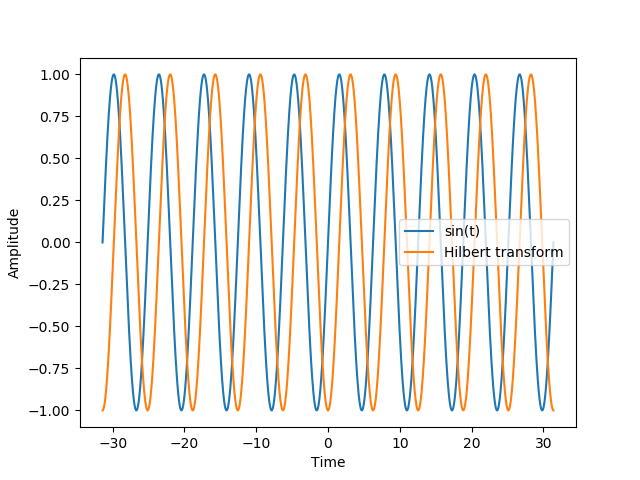
\includegraphics[width=0.8\linewidth]{../fig/h_sin}
	\caption{The Hilbert transform of $\sin(ct)$ given by $\sin(ct-\frac{\pi}{2})$. $c=1$  }
	\label{fig:hsin}
\end{figure}
\justify
Figure \ref{fig:hsin} shows the Hilbert transform of $\sin(ct)$ which is $\sin\left(ct-\frac{\pi}{2}\right)$. In the same fashion, the Hilbert transform of $\cos(ct)$ is  $\cos\left(ct-\frac{\pi}{2}\right)$, where $c = 1$. Therefore, in the frequency domain, the Hilbert transform imposes a phase shift of $\frac{\pi}{2}$ to every Fourier component of a signal. 
\begin{figure}[H]
	\centering
	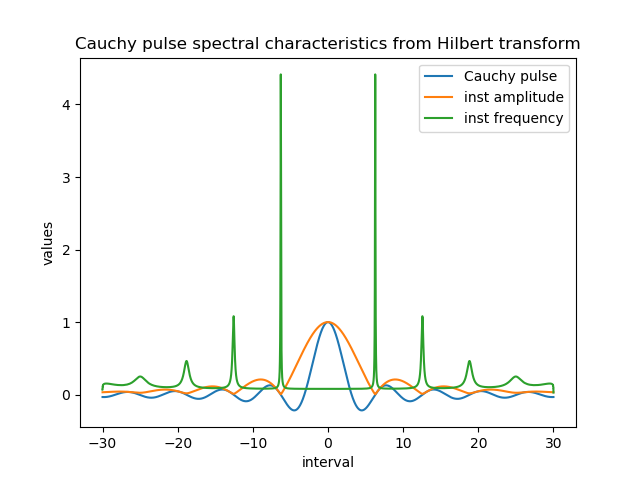
\includegraphics[width=1\linewidth]{../fig/cauchy_pulse_spectral}
	\caption{Cauchy pulse with its instantaneous (inst) amplitude and frequency. $c=1$}
	\label{fig:cauchy_pulse}
\end{figure}
\justify
Figure \ref{fig:cauchy_pulse} shows the Cauchy pulse, which is given by ($c=1$)
\begin{equation}
	 \frac{c}{c^{2}+ t^{2}},
\end{equation}
as well as its instantaneous (inst) amplitude and frequency on the interval $[-30, 30]$. Considering the Cauchy pulse on the time interval $[0,30]$, its amplitude and frequency decay in time. This is well captured by the instantaneous amplitude and frequency in Figure \ref{fig:cauchy_pulse}.
\justify
Le further illustrate the importance of the Hilbert transform for frequency and amplitude modulated signals. This example is taken from (\cite{scipy2019}), the official page of the Python implementation of the Hilbert transform. It depicts the strength, as well as the short coming of the Hilbert transform. Consider the signal given in Figure \ref{fig:mode}. 

\begin{figure}[H]
	\centering
	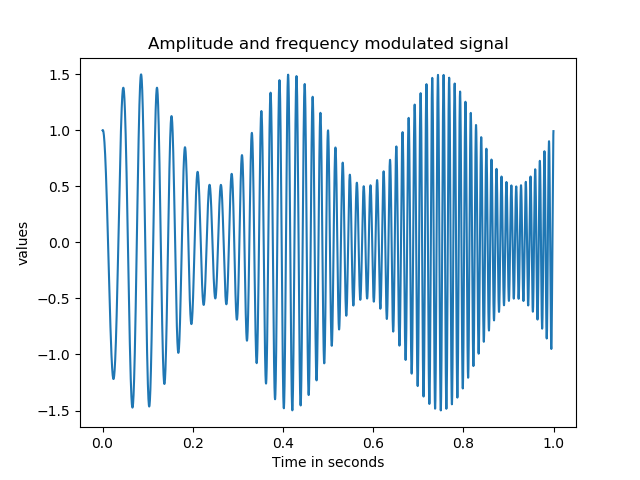
\includegraphics[width=1\linewidth]{../fig/mode}
	\caption{A signal with amplitude and frequency variation in time}
	\label{fig:mode}
\end{figure}
\justify
As one can can observe, its frequency changes from 20 Hz to 100 Hz from 0 to 1 second, while its amplitude varies in time. By computing its Hilbert transform, the signal is extended to the upper complex plane, as an analytic signal. Therefore using (\ref{eq:amplitude}-\ref{eq:phase}), its instantaneous frequency and amplitude can be computed.
\justify
Figure \ref{fig:inst} shows the corresponding instantaneous amplitude and frequency. It is clear from this that the frequency changes (nearly) from 20 Hz in the neighborhood of $t=0$, to 100 Hz in the neighborhood of $t = 1$ . This demonstrates the efficiency of the Hilbert transform in dealing with signals with modulated spectral characteristics. 
\justify
Although the Hilbert transform provides a tool to analyze signals with modulated spectral characteristics, the instantaneous frequency obtained does not always provide a physical meaning (\cite{huang98}, \cite{huang08}). As one can observe in Figure \ref{fig:inst}, at the endpoints of the interval $[0,1]$, the instantaneous frequency is not a single-valued function of time. It means that at a single point in time, multiple frequency values are defined. This obviously violate physical laws. The explanation as to why this occurred, is found in the signal not being mono-component. That is, the target signal is a superposition of elementary sub-signals.
\begin{figure}[H]
	\centering
	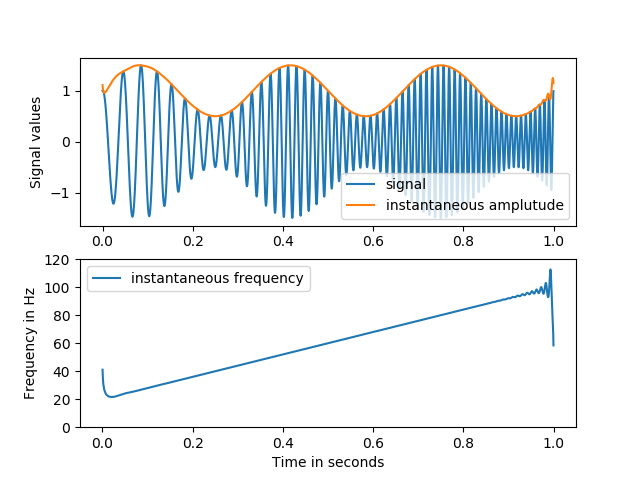
\includegraphics[width=1\linewidth]{../fig/inst}
	\caption{A signal with amplitude and frequency variation in time}
	\label{fig:inst}
\end{figure}
\justify
Formally, a mono-component signal say $z(t)$ has an analytic (complex) representation 
\begin{equation}
	z(t) = a(t)e^{i \Psi(t)} 
\end{equation}
where $a(t)$ and $\Psi(t)$ are the instantaneous amplitude and phase respectively,
and the pair $a(t)$, $e^{i \Psi(t)}$ are spectrally disjoint.
\justify
 To address the issue faced by the Hilbert transform for non mono-component signals, the Hilbert-Huang transform was developed. Through the so called empirical mode decomposition (EMD), which is a series of transformation, a target signal is decomposed into (nearly) mono-component signals called intrinsic mode function, for which instantaneous amplitude and frequency are well defined in a physical sense. Therefore, the Hilbert Huang transform adds value to the Hilbert transform, and both make it possible to correctly tackle problems with frequency and amplitude modulation. A concise exposition of the Hilbert-Huang transform is given in chapter 3, where it is applied in a proposed new method, for bearing fault detection. 
\justify
To sum up: The Hilbert transform acts as a linear filter in the frequency domain, where it imposes a phase shift to every Fourier component. In the time domain, it extends a real valued function to a complex function which is an analytic signal. The imaginary part of the latter is the Hilbert transform of the original signal. By using the analytic signal, the instantaneous frequency and the instantaneous amplitude of the original signal is derived. To have a meaning instantaneous amplitude and frequency, the original signal must be a mono-component signal, meaning that it must not be the superposition of signals. The Hilbert Huang transform, makes it possible to decompose any signal to a set of (nearly) mono-components signals called intrinsic mode function. Thus, the Hilbert transform, coupled with the Hilbert Huang transform provide a complete set of tools, in analyzing frequency and amplitude modulated signals.
  


%%%%%%%%%%%%%%%%%%%%%%%%%%%%%%%%%%%%%%%%%%%%%%%%%%%%%%%%%%%%%%%%%%%%%%%%%%%%%%
%\subsubsection{Lowpass and highpass filter}
%\label{sec:other-filters}


\clearpage
%%%%%%%%%%%%%%%%%%%%%%%%%%%%%%%%%%%%%%%%%%%%%%%%%%%%%%%%%%%%%%%%%%%%%%%%%%%%%%%%%%%%%
%%%%%%%%%%%%%%%%%%%%%%%%%%%%%%%%%%%%%%%%%%%%%%%%%%%%%%%%%%%%%%%%%%%%%%%%%%%%%%%%%%%%%


\section{Application of the high frequency resonance technique for bearing fault detection}
\label{sec:application}
In the literature review section, the high frequency resonance techniques (HFRT) was presented as one of the most widely used method for bearing fault detection. In this section, the HFRT is applied to a case study, which consists of detecting defects in the outer and inner ring of a roller bearing.
\justify
Section \ref{sec:case} describes the experimental set up that generated the bearings vibration signals for this case study. In section \ref{sec:fault} the theoretical equations for bearing defects frequencies are formulated. Furthermore, the characteristics of each fault are described.
Finally, the results from applying the high frequency resonance technique are presented in section \ref{sec:method}.


%%%%%%%%%%%%%%%%%%%%%%%%%%%%%%%%%%%%%%%%%%%%%%%%%%%%%%%%%%%%%%%%%%%%%%%%%%%%%%%%%%%%%%%%%%%%%%%%%%%%%%%%%%%%%%%%%%%%%%%
\subsection{Description of the case study}
\label{sec:case}
The data for this case study was generated by the Intelligence Maintenance System (IMS), at the University of Cincinnati. It is freely available online and was measured by (\cite{lee2007}). It has been the subject of numerous publications such as 
(\cite{hai2006}, \cite{mejia2010}, \cite{fangtao2011}, \cite{mejia2011}, \cite{mortada2011}, \cite{rego2011}, \cite{yacout2012}, \cite{sergey2012} , \cite{of2012}, \cite{jianbo2012a}, \cite{jianbo2012b}, \cite{mejia2012} )
\justify
Three separate experiments involving four bearings were performed on a motor. In each experiment, a one second vibration signal snapshot was recorded every five or ten minutes. Each vibration signal (sample), consists of 20 480 data points with a sampling rate of 20 000 Hz.
The sampling rate also called sampling frequency, is the average number of sample points obtained per second during the sampling process. The sampling process is the reduction of an analog signal to a digital signal. The analog signal is the continuous time signal, while the digital signal is the discrete time signal of interest. The experimental set up is shown in Figure \ref{fig:exp} where
\begin{figure}[H] %  figure placement: here, top, bottom, or page
   \centering
   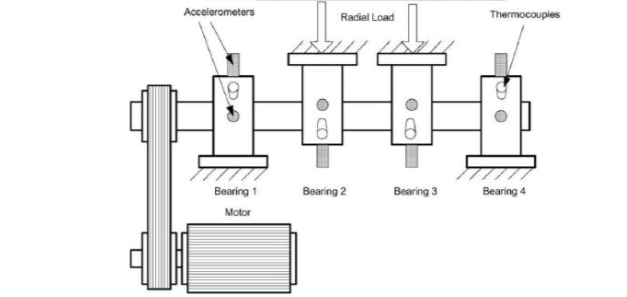
\includegraphics[width=7in]{../fig/experiment} 
   \caption{Experimental set up.}
   \label{fig:exp}
\end{figure}
\justify
four bearings support a rotating shaft, driven by an AC motor through rub belts. The motor rotates at 2000 rotations per minute, while the bearings are subjected to a constant radial force of 6000 pounds. In the first experiment two accelerometers were mounted on the bearings. Each measuring vibration for the axial and radial position respectively.
In the second and third experiment, four accelerometers were placed one each bearing, measuring axial vibration.
Recall that an accelerometer is a sensor that measures vibration signals, in particular the acceleration experienced by the bearings in this case. Axial signals are measured along the axis of the motor shaft, while radial signals are measured along the perpendicular direction of the motor shaft.
\justify
At the end of the first experiment, an inner race defect occurred in bearing number 3 and a roller element defect occurred in bearing number 4. At the end of the second experiment, an outer race defect occurred in bearing number 1 and 3, respectively. 

%%%%%%%%%%%%%%%%%%%%%%%%%%%%%%%%%%%%%%%%%%%%%%%%%%%%%%%%%%%%%%%%%%%%%%%%%%%%%%%%%%%%%
%%%%%%%%%%%%%%%%%%%%%%%%%%%%%%%%%%%%%%%%%%%%%%%%%%%%%%%%%%%%%%%%%%%%%%%%%%%%%%%%%%%%%


\subsection{Bearing defects}
\label{sec:fault}
As pointed out earlier, bearing failure frequencies depend on their physical characteristics and the rotating speed of the motor housing them. Figure \ref{fig:bearing} shows a graphical representation of a bearing, with the outer ring, the cages that encircle the balls (rolling elements), and the inner ring, where the motor shaft is attached.
\begin{figure}[H] %  figure placement: here, top, bottom, or page
   \centering
   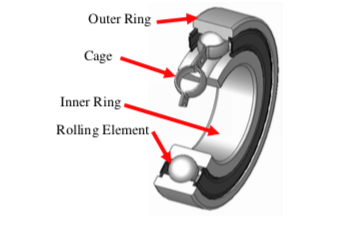
\includegraphics[width=3.2in]{../fig/bearing}  
   \caption{Geometrical view of a bearing}
   \label{fig:bearing}
\end{figure}
\justify
 an inner ring defect occurs at a frequency called ball pass frequency inner race (BPFI), while an outer race defect occurs at a frequency call ball pass outer race frequency (BPFO). They are expressed in Hz in terms of the bearing geometry characteristics and the shaft rotation speed as 
\begin{equation}\label{eq:bpfi}
BPFI = \frac{nb}{2}S\left( 1 +  \frac{BD}{PD}\cos(\beta)  \right)
\end{equation}

\begin{equation}\label{eq:bpfo}
BPFO = \frac{nb}{2}S\left( 1 -  \frac{BD}{PD}\cos(\beta)  \right)
\end{equation}
where 
\begin{itemize}
\item S is the rotating speed of the motor
\item nb is the number of cylindrical balls (roller elements)
\item BP is the the ball diameter
\item PD is the pitch diameter
\item $\beta$ is the contact angle
\end{itemize}
The pitch diameter is the perpendicular distance from the center of one ball to the center of the ball located at the end.
The bearing type used in this experiment are manufactured by the company Rexnord, and are of type Rexnord ZA 2115, with BPFO and BPFI given by 236.4 Hz, 296.8 Hz respectively. 
%%%%%%%%%%%%%%%%%%%%%%%%%%%%%%%%%%%%%%%%%%%%%%%%%%%%%%%%%%%%%%%%%%%%%%%%%%%%%%%%%%%%%
%%%%%%%%%%%%%%%%%%%%%%%%%%%%%%%%%%%%%%%%%%%%%%%%%%%%%%%%%%%%%%%%%%%%%%%%%%%%%%%%%%%%%


\subsection{High frequency resonance technique application to failure detection}
\label{sec:method}
The high frequency resonance technique consists of a series of operation whose goal is to extract frequency component from a time signal.
There are four steps in transforming a time signal into frequency spectrum: A band pass filtering, enveloping, a low pass filtering and a fast Fourier transformation.
Figure \ref{fig:fft-process} shows a schematic description of the entire process. 
\justify
The band pass filter process allows signals within a prescribed frequency band to seep through, while attenuating non essential signals. The band of allowed frequencies is bounded bellow and above by two parameters: The low cut-off frequency and the high cut-off frequency, respectively. In this application a low cut-off frequency of 2000 Hz and a high cut-off frequency of 9990 Hz were used.
%The intent is to only capture bearing vibration signal and ignore any other. Once this done, the demodulation extract the high frequency time domain signal and a low pass filter extract the low frequency. The Fast Fourier transform is then applied to the time domain signal to generate the frequency spectrum.
\begin{figure}[H]
\begin{tikzpicture}
  [node distance=.8cm,
  start chain=going below,]
     \node[punktchain, join] (intro) {Signal};
     \node[punktchain, join] (probf)      {Band pass filtering};
     \node[punktchain, join] (investeringer)      {Hilbert transform'5};
     \node[punktchain, join] (perfekt) {Low pass filtering};
     \node[punktchain, join, ] (emperi) {Fast Fourier transform};
     % \node (asym) [punktchain ]  {Asymmetrisk information};
      \begin{scope}[start branch=venstre,
        %We need to redefine the join-style to have the -> turn out right
        every join/.style={->, thick, shorten <=1pt}, ]
        \node[punktchain, on chain=going left, join=by {->}] (risiko) {Frequency spectrum};
      \end{scope}
      \begin{scope}[start branch=hoejre,]
      %\node (finans) [punktchain, on chain=going right] {Det finansielle system};
    \end{scope}
    \end{tikzpicture}
  \caption{Description of the high frequency resonance technique.}
   \label{fig:fft-process}
\end{figure}
\justify
%The enveloping step corresponds to rectifying the signal. It accounts only for the positive part of the signal, and extract the high frequency resonance component induced by bearing defects, and the defect characteristics frequency component.
%\justify
%In mathematically terms, the envelope  $E(t)$ of a signal $x(t)$ is given by
%\begin{equation}
%E(t) = \sqrt{H(t)^{2}+ x(t)^{2}}
%\end{equation}
%were 
%\begin{equation}
%H(t) = \frac{1}{\pi t}*x(t) = \frac{1}{\pi}\int_{-\infty}^{+\infty}\frac{x(t)}{t-\tau}\mathrm{d}\tau
%\end{equation}
%is the Hilbert transform of the signal, and \say{*} define the convolution operation.
% After the enveloping process, the resulting signal is low pass filtered in order to remove the high frequency resonance components, leaving only the signal component that contain the bearing failure frequencies. Finally, the fast Fourier transform is applied on the filtered signal to obtain the frequency spectrum.
%%%%%%%%%%%%%%%%%%%%%%%%%%%%%%%%%%%%%%%%%%%%%%%%%%%%%%%%%%%%%%%%%%%%%%%%%%%%%%%%%%%%%
%%%%%%%%%%%%%%%%%%%%%%%%%%%%%%%%%%%%%%%%%%%%%%%%%%%%%%%%%%%%%%%%%%%%%%%%%%%%%%%%%%%%%
\subsubsection{Ball pass outer race defect frequency detection}
%
\begin{figure}[H]
	\centering
	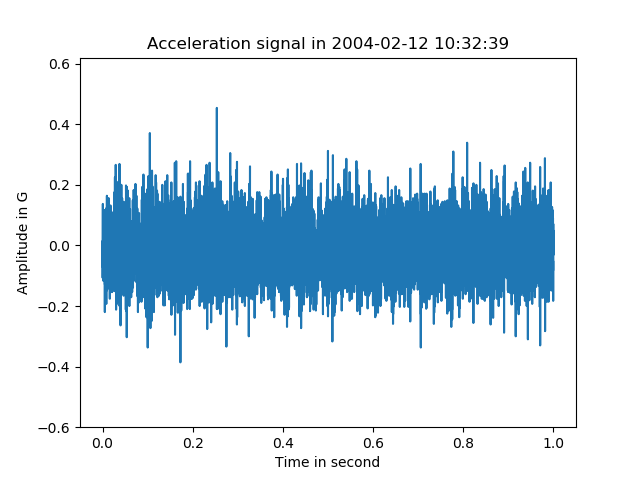
\includegraphics[width=0.7\linewidth]{../fig/bpfo/first_day_signal_bpfo}
	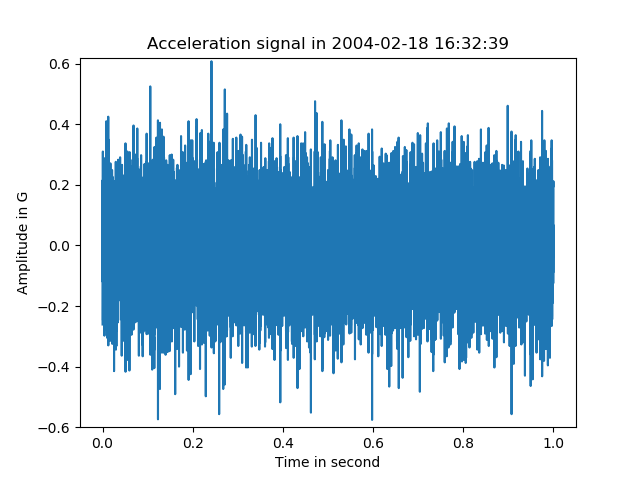
\includegraphics[width=0.7\linewidth]{../fig/bpfo/last_day_signal_bpfo}
	\caption{Vibration time signals of bearing number 1 recorded at the beginning (top) and six days after (bottom), in experiment 2.}
	\label{fig:bpfo_signal}
\end{figure}
In experiment 2, four bearings were run to failure, resulting in outer race defect in bearing  number 1.
Figure \ref{fig:bpfo_signal} shows the vibration time signals of bearing number 1, at the beginning (top) and six days after (bottom), from experiment number 2. A significant increase in the variance can be observed.
I fact, the variance has increased 28 time after 6 days. This can be seen in Figure \ref{fig:bpfo_density}, which shows a density plot at the beginning and six days after.
\begin{figure}[H]
	\centering
	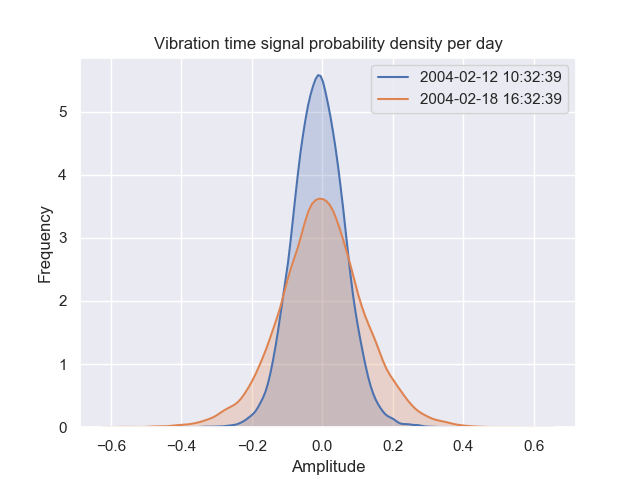
\includegraphics[width=0.7\linewidth]{../fig/bpfo/density_bpfo_signal}
	\caption{Density plot of the time signal at the beginning and six days after}
	\label{fig:bpfo_density}
\end{figure}
\justify
After six days, the tail of the distribution increases considerably, which indicates an increase in the variance, due to bearing defect propagation. Figure \ref{fig:bpfo} shows the corresponding frequency spectrum at the beginning (top) and six days after (bottom). At the beginning of the experiment, the frequency spectrum is relatively \say{clean}. No high frequency peaks can be observed. This indicates that the bearing is relatively \say{healthy}. However, after six days, the ball pass frequency as well as harmonics can be observed in the frequency spectrum.
\justify
Harmonics are evenly spaced frequency peaks that are integer multiple of the ball pass outer race defect frequency (\cite{mobius2014}). They are indication of transient, clipping or random impact in the vibration signal, and are characteristics of the presence of bearing defects (\cite{mobius2014}). Transient indicates the variation of the signal properties with time, while clipping refers to the distortion of a signal. 
\justify
 Figure \ref{fig:experiment2_bearing_fft_amp} shows the evolution of defect frequency in terms of amplitude as a function of time, for all  bearings. Clearly, bearing 1 exhibits high amplitude in terms of defect frequency compare to other bearings. Its amplitude increases and drops, before increasing in an oscillatory fashion. This is due to random slip or clipping caused by defect propagation in the bearing. This illustrates the fact that the vibration signal generated by bearing are non periodic and stochastic (\cite{randal2011}).
\begin{figure}[H]
	\centering
	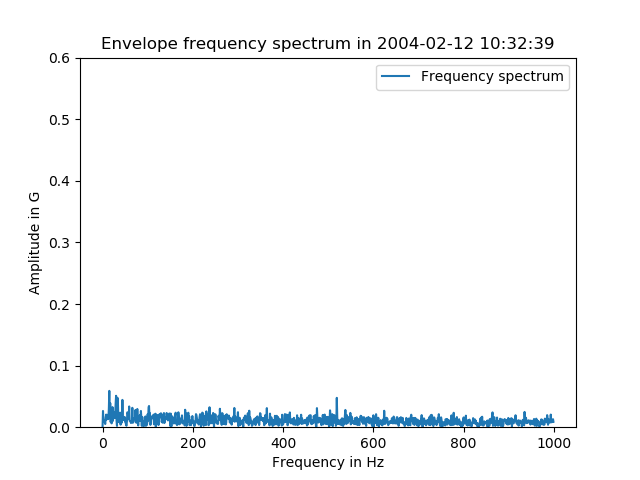
\includegraphics[width=0.7\linewidth]{../fig/bpfo/first_day_spectrum_bpfo}
	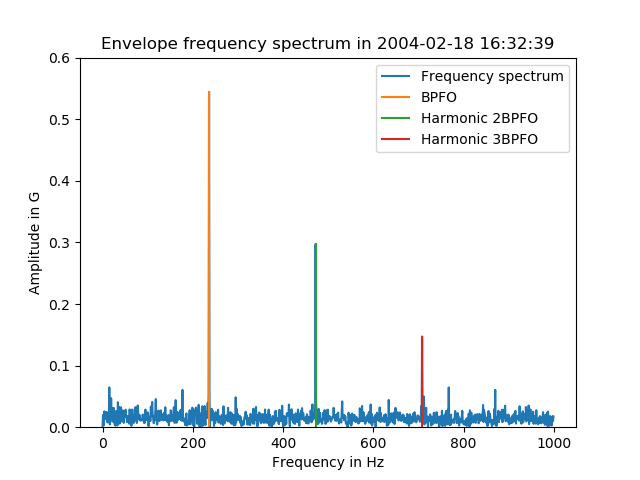
\includegraphics[width=0.7\linewidth]{../fig/bpfo/last_day_spectrum_bpfo}
	\caption{Frequency spectrum with the presence of outer race defect frequency and harmonics.}
	\label{fig:bpfo}
\end{figure}

\begin{figure}[H] 
   \centering
    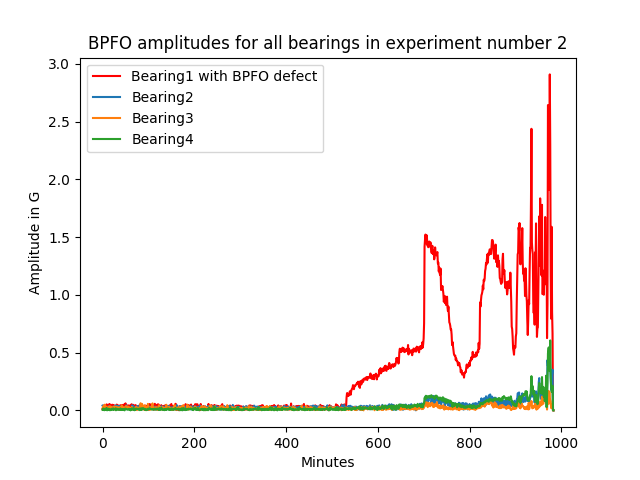
\includegraphics[width=4.9in]{../fig/experiment2_bearing_fft_amp.png}
  % 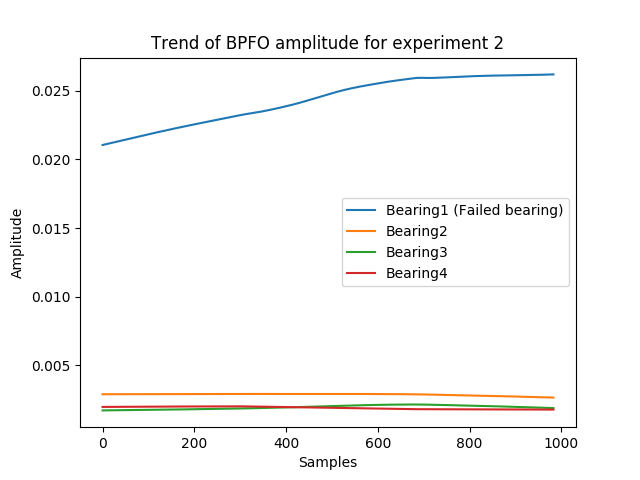
\includegraphics[width=4.4in]{../fig/experiment2_bearing_fft_trend.png} 
   \caption{BPFO amplitude evolution for all bearings over time}
   \label{fig:experiment2_bearing_fft_amp}
\end{figure}
\clearpage

\subsubsection{Ball pass inner race defect frequency detection}
Recall that in experiment 1, four bearings were run to failure, and at the end of the experiment, inner race defect occurred in bearing number 3. Figure \ref{fig:bpfi_signal} shows the vibration signals of bearing number 3, at the beginning (top) and at the end (bottom) of the experiment.
\begin{figure}[H]
	\centering
	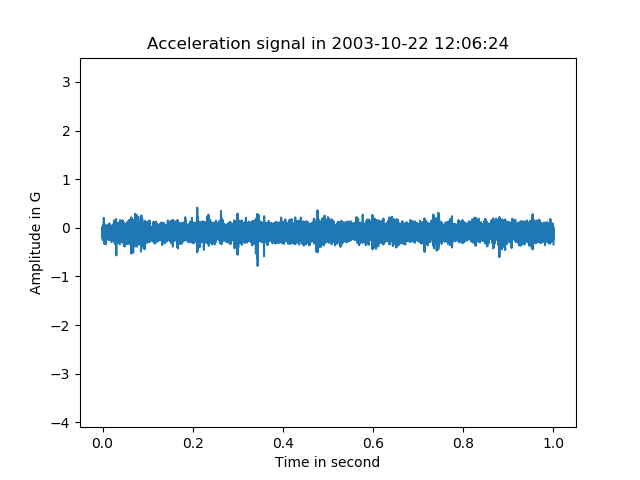
\includegraphics[width=0.7\linewidth]{../fig/bpfi/first_day_signal}
	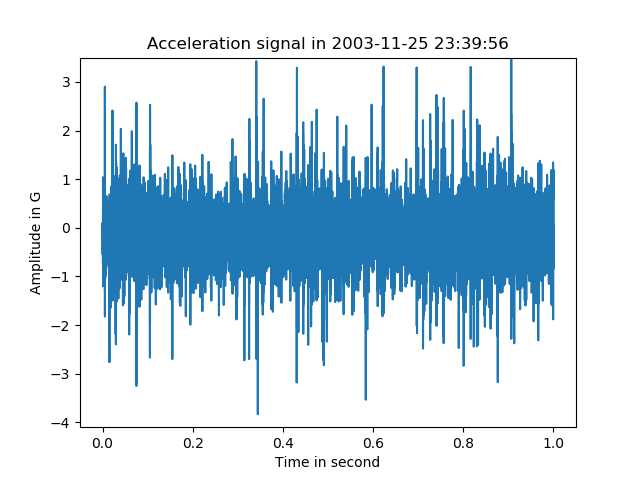
\includegraphics[width=0.7\linewidth]{../fig/bpfi/last_day_signal}
	\caption{Vibration time signals recorded at the beginning (top) and at the end (bottom), of experiment 1.}
	\label{fig:bpfi_signal}
\end{figure}


\begin{figure}[H]
	\centering
	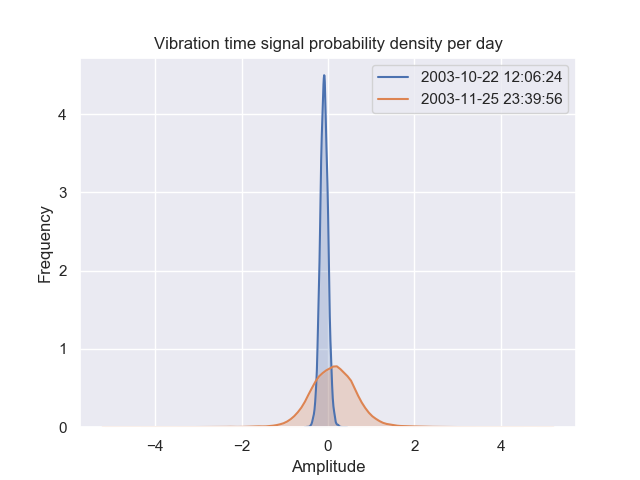
\includegraphics[width=0.7\linewidth]{../fig/bpfi/bpfi_density}
	\caption{Density plot of the time signal at the beginning and at the end of the experiment 1, for bearing number 3.}
	\label{fig:bpfi_density}
\end{figure}
\justify
It is clear that the variance of the time signal had increased significantly. This can be seen from the density plot in Figure \ref{fig:bpfi_density}, where the distribution of the signal at the end of the experiment exhibits a pronounced wide tail. In fact, the variance had increased 41 time its initial value. The frequencies spectrum at the beginning (top) and at the end (bottom) of the experiment can be seen in Figure \ref{fig:bpfi}. The frequency spectrum at the beginning of the experiment does not contain any high peaks frequencies. It is completely \say{clean}. This means that the bearing is relatively \say{healthy}.
\justify
However, at the end of the experiment, the frequency spectrum exhibits a ball pass inner race frequency and form sidebands together with surrounding peaks.
Sidebands are series of (almost) evenly spaced frequency peaks, centered around a center peak called carrier (\cite{mobius2014}).
They are result of amplitude modulation between the shaft frequency and the ball pass inner race defect frequency (\cite{mobius2014}). This is due to the fact that the inner race fault will rotate in and out of the loaded region, causing modulation of the impact amplitudes by the rotation speed of the shaft (\cite{courrech}).
\begin{figure}[H]
	\centering
	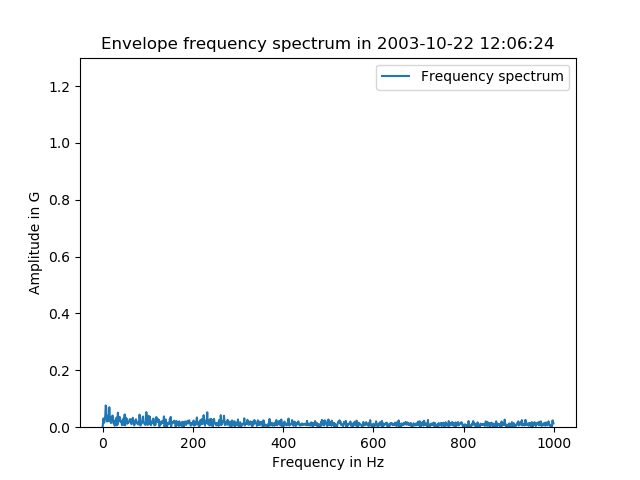
\includegraphics[width=0.7\linewidth]{../fig/bpfi/first_day_spectrum}
	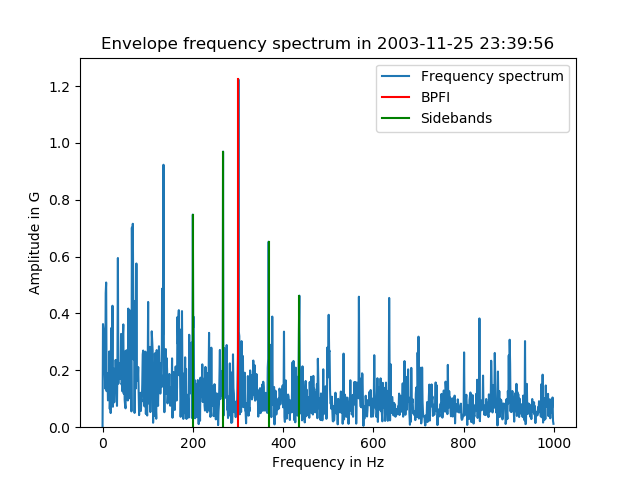
\includegraphics[width=0.7\linewidth]{../fig/bpfi/bpfi_sidebands}
	\caption{Frequency spectrum with the presence of inner race defect frequency and sidebands.}
	\label{fig:bpfi}
\end{figure}
\justify
The high frequency resonance technique applied to inner race defect detection, can produce a confusion spectrum, with pattern of spectral line changing (\cite{mcfadden1984a}). This make identifying inner race defect difficult in situation where the defect is pronounced. In those cases the defect frequency values can vary up to $2\%$ (\cite{randal2010}). Although the rotating speed of the machine is set as a constant value, in practice however, there is always small variations, that will also generate a variation in the theoretical value of the frequency defect.


\clearpage
\section{Summary}
\label{sec:chapter_conclusion}
Fourier analysis applied to bearing fault detection, is concerned with transforming the vibration time signal of a bearing, to its corresponding frequency spectrum. A defect generates an impulse, which induces resonance in the bearing, and the machine housing the bearing. The generated resonance represents the response of the former and the latter.
\justify
The diagnostic information for bearing fault detection resides in the high frequency resonance induced by defects. The latter are frequency components, expressed mathematically in terms of the bearings physical characteristics, and the rotational speed of the machine shaft. The most prevalent technique used to extract bearing diagnostic information is the high frequency resonance technique.
\justify
The latter uses a series of filtering operations, aiming at isolating the bearing signal containing the failure frequencies. Furthermore, the frequency spectrum is extracted from the time signal through Fourier transform. If defects are initiated, the frequency spectrum will contain the defects frequencies. Although efficient, the high frequency resonance technique is only valid within the boundary of the assumptions upon which it is predicated. 
\justify
Due to slip of the roller elements in the bearing, the failure frequencies values can vary up to 2$\%$ from their theoretical values, or even more. In addition, bearing signal are relatively non periodic and stochastic in nature. Consequently, non-stationarity and non-linearity can be observed in bearing signal. The dependency of the failure frequency on the rotation speed of the machine shaft is also a limiting factor. For unknown or inaccurate rotation speed, the detection of failure become unreliable, or even impossible. The need for alternative methods for bearing fault detection is therefore justified and imperative. In particular, method that does not only rely on the frequency spectrum are important. In the next chapters, such methods are presented.



















\blankpage
\end{document}

